\documentclass[11pt]{article}

\usepackage[margin=1in]{geometry}
\usepackage[T1]{fontenc}
\usepackage{lmodern}

\usepackage{amsmath, amssymb}

\usepackage{setspace}

\usepackage[most]{tcolorbox}
\usepackage{xcolor}

\tcbset{
  enhanced,
  boxrule=0pt,
  frame hidden,
  breakable
}

\usepackage{fancyhdr}
\pagestyle{fancy}
\fancyhf{}
\setlength{\headheight}{52pt}
\renewcommand{\headrulewidth}{0pt}

\usepackage{tikz}
\usetikzlibrary{arrows.meta}
\usetikzlibrary{calc}

\newcommand{\Course}{Math 4610 Spring 2026}
\newcommand{\Instructor}{Homework 6}
\newcommand{\AssignmentType}{Homework} % or Discussion
\newcommand{\AssignmentNumber}{6}

\newcommand{\Contributors}{
Marks, Stephen
}

\fancyhead[L]{\Course\\ \Instructor}
\fancyhead[R]{\Contributors}

\newcommand{\ProblemDivider}[1]{%
  \vspace{1.0em}
  \noindent\textbf{#1}\par
  \vspace{0.35em}
}

\definecolor{problemBack}{RGB}{235,242,250}
\definecolor{problemFrame}{RGB}{70,110,160}
\definecolor{exerciseGray}{gray}{0.96}
\definecolor{exerciseGrayFrame}{gray}{0.45}

\newtcolorbox{problemBox}{
  colback=exerciseGray,
  colframe=exerciseGrayFrame,
  arc=2mm,
  left=8pt,right=8pt,top=8pt,bottom=8pt
}

\newtcolorbox{solutionBox}{
  colback=white,
  colframe=white,
  arc=0mm,
  left=0pt,right=0pt,top=0pt,bottom=0pt
}

\newcommand{\ProblemAnnounce}{\noindent}
\newcommand{\SolutionAnnounce}{\noindent\textbf{Solution.}\par\medskip}

\newcommand{\Exercise}[1]{\textbf{Exercise~#1.}\;}

\newcommand{\R}{\mathbb{R}}
\newcommand{\C}{\mathbb{C}}
\newcommand{\<}{\langle}
\renewcommand{\>}{\rangle}
\newcommand{\norm}[1]{\|#1\|}

\begin{document}

\begin{center}
  {\Large \textbf{\AssignmentType~\AssignmentNumber}}
\end{center}
\vspace{0.75em}

\ProblemDivider{1}

\begin{problemBox}
\ProblemAnnounce
\Exercise{6.A.33}
Suppose $f, g$ are differentiable functions from $\R$ to $\R^n$.
\begin{enumerate}
  \item[(a)] Show that
  \[\<f(t), g(t)\>' = \<f'(t), g(t)\> + \<f(t), g'(t)\>.\]
  \item[(b)] Suppose $c$ is a positive number and $\|f(t)\| = c$ for every $t \in \R$. Show that
  $\<f'(t), f(t)\> = 0$ for every $t \in \R$.
  \item[(c)] Interpret the result in (b) geometrically in terms of the tangent vector to a curve
  lying on a sphere in $\R^n$ centered at the origin.
\end{enumerate}
\end{problemBox}

\begin{solutionBox}
\SolutionAnnounce
\doublespacing

\begin{enumerate}
  \item[(a)] Suppose that $f(t) = (f_1(t), \ldots, f_n(t))$ and $g(t) = (g_1(t), \ldots, g_n(t))$ for some differentiable
  functions $f_1, \ldots, f_n, g_1, \ldots, g_n: \R \to \R$. By the standard rules of differentiation we have
  \[
  \begin{aligned}
  \<f(t), g(t)\>' &= (f_1(t)g_1(t) + \cdots + f_n(t)g_n(t))' \\
  &= f_1'(t)g_1(t) + f_1(t)g_1'(t) + \cdots + f_n'(t)g_n(t) + f_n(t)g_n'(t) \\
  &= f_1'(t)g_1(t) + \cdots + f_n'(t)g_n(t) + f_1(t)g_1'(t) + \cdots + f_n(t)g_n'(t) \\
  &= \<f'(t), g(t)\> + \<f(t), g'(t)\>.
  \end{aligned}
  \]
  
  \item[(b)] By part (a) we have
  \[
  0 = (c^2)' = (\|f(t)\|^2)' = \<f(t), f(t)\>' = 2\<f'(t), f(t)\>.
  \]
  Thus $\<f'(t), f(t)\> = 0$.
  
  \item[(c)] Suppose $c > 0$. A differentiable function $f: \R \to \R^n$ satisfying $\|f(t)\| = c$ for every
  $t \in \R$ traces a curve which lies on a sphere of radius $c$ centered at the
  origin in $\R^n$. The tangent vector to this curve is given by $f'$. By part (b)
  this tangent vector is always orthogonal to the position vector $f(t)$. So the tangent line is perpendicular to the radius at each point on the sphere.
\end{enumerate}
\end{solutionBox}

\ProblemDivider{2}

\begin{problemBox}
\ProblemAnnounce
\Exercise{6.A.34}
Use inner products to prove Apollonius's identity: In a triangle with
sides of length $a$, $b$, and $c$, let $d$ be the length of the line segment from the midpoint of
the side of length $c$ to the opposite vertex. Then
\[a^2 + b^2 = \frac{1}{2}c^2 + 2d^2.\]
\end{problemBox}

\begin{solutionBox}
\SolutionAnnounce
\doublespacing

Consider the following triangles formed by vectors:

\begin{center}
\begin{tikzpicture}[>=Stealth, line cap=round, line join=round, scale=1.15]

    \fill[gray!15] (-0.8,-0.8) rectangle (10.8,5.2);

    \coordinate (A) at (1.5,0);
    \coordinate (B) at (3.5,0);
    \coordinate (C) at (5.5,0);
    \coordinate (D) at (6.8,4.8);
    \coordinate (E) at (8.9,4.8);

    \draw[->, very thick] (A) -- (B);
    \draw[->, very thick] (B) -- (C);

    \draw[->, very thick] (A) -- (D);
    \draw[->, very thick] (B) -- (D);
    \draw[->, very thick] (C) -- (D);

    \draw[->, very thick, dotted] (D) -- (E);
    \draw[->, very thick, dotted] (C) -- (E);

    \node[below] at ($(A)!0.5!(B)$) {$v$};
    \node[below] at ($(B)!0.5!(C)$) {$v$};

    \node at (4.0,2.5) {$u$};
    \node at (4.4,2.0) {$u-v$};
    \node at (5.4,1.55) {$u-2v$};

\end{tikzpicture}
\end{center}

Then
\[\|u\| = a,\quad \|v\| = \frac{1}{2}c,\quad \|u-v\| = d,\quad \|u-2v\| = b.\]

Observe the parallelogram formed by the vectors $u-v$ and $v$. The parallelogram equality
states that
\[\|u\|^2 + \|u-2v\|^2 = 2\|v\|^2 + 2\|u-v\|^2.\]

Then by substitution,
\[a^2 + b^2 = \frac{1}{2}c^2 + 2d^2.\]
\end{solutionBox}
\newpage

\ProblemDivider{3}

\begin{problemBox}
\ProblemAnnounce
\Exercise{6.B.7}
Suppose $T \in \mathcal{L}(\R^3)$ has an upper-triangular matrix with respect to
the basis $(1, 0, 0)$, $(1, 1, 1)$, $(1, 1, 2)$. Find an orthonormal basis of $\R^3$ with respect to
which $T$ has an upper-triangular matrix.
\end{problemBox}

\begin{solutionBox}
\SolutionAnnounce
\doublespacing

Performing the Gram-Schmidt procedure on the basis $(1, 0, 0)$, $(1, 1, 1)$, $(1, 1, 2)$
yields the orthonormal basis
\[\left(1, 0, 0\right),\quad \left(0, \frac{1}{\sqrt{2}}, \frac{1}{\sqrt{2}}\right),\quad \left(0, -\frac{1}{\sqrt{2}}, \frac{1}{\sqrt{2}}\right).\]

The matrix of $T$ with respect to this orthonormal basis must also
be upper-triangular by 6.37.
\end{solutionBox}

\ProblemDivider{4}

\begin{problemBox}
\ProblemAnnounce
\Exercise{6.C.3}
Suppose $U$ is the subspace of $\R^4$ defined by
\[U = \text{span}((1, 2, 3, -4), (-5, 4, 3, 2)).\]
Find an orthonormal basis of $U$ and an orthonormal basis of $U^\perp$.
\end{problemBox}

\begin{solutionBox}
\SolutionAnnounce
\doublespacing

We can verify that
\[u_1 = (1, 2, 3, -4),\ u_2 = (-5, 4, 3, 2),\ v_1 = (1, 0, 0, 0),\ v_2 = (0, 1, 0, 0)\]
is a basis of $\R^4$ as they are 4 linearly independent vectors in $\R^4$. And $u_1, u_2$ is a basis of $U$. Performing the Gram-Schmidt procedure
on this list yields the orthonormal list
\[
\begin{aligned}
e_1 &= \frac{1}{\sqrt{30}}(1, 2, 3, -4),\\
e_2 &= \frac{1}{\sqrt{12030}}(-77, 56, 39, 38),\\
f_1 &= \frac{1}{\sqrt{76190}}(190, 117, 60, 151),\\
f_2 &= \frac{1}{9\sqrt{190}}(0, 81, -90, 27).
\end{aligned}
\]

So $e_1, e_2$ must be an orthonormal basis of $U$ and $f_1, f_2$ must
be an orthonormal basis of $U^\perp$.
\end{solutionBox}

\ProblemDivider{5}

\begin{problemBox}
\ProblemAnnounce
\Exercise{6.C.15}
In $\R^4$, let
\[U = \text{span}((1, 1, 0, 0), (1, 1, 1, 2)).\]
Find $u \in U$ such that $\|u - (1, 2, 3, 4)\|$ is as small as possible.
\end{problemBox}

\begin{solutionBox}
\SolutionAnnounce
\doublespacing

Let $u_1 = (1, 1, 0, 0)$ and $u_2 = (1, 1, 1, 2)$, so that $u_1, u_2$ is a basis of $U$. Performing
the Gram-Schmidt procedure on the list $u_1, u_2$ yields the list
\[e_1 = \frac{1}{\sqrt{2}}(1, 1, 0, 0),\quad e_2 = \frac{1}{\sqrt{5}}(0, 0, 1, 2),\]
which is an orthonormal basis of $U$. Let $v = (1, 2, 3, 4)$. By 6.61, to minimize $\|u - v\|$
we should take $u = P_U v$. This can be calculated by 6.57(i):
\[P_U v = \<v, e_1\>e_1 + \<v, e_2\>e_2 = \left(\frac{3}{2}, \frac{3}{2}, \frac{11}{5}, \frac{22}{5}\right).\]
\end{solutionBox}

\end{document}
